This chapter describes the theoretical framework which the analysis presented in the dissertation is based on. The Standard Model (SM) is briefly described in~\cref{sec:sm} along with its limitations in the form of inability to explain observed anomalies.~\Cref{sec:hnl} introduces a family of Beyond Standard Model (BSM) particles, Heavy Neutral Leptons (HNLs), proposed to explain some of these anomalies. HNLs form the benchmark model probed in this search.

\section{Standard Model}\label{sec:sm}
The Standard Model is our best understanding of the particulate nature of the universe at the most fundamental level. The theory\footnote{The description of the Standard Model is adapted from the book ``Quarks and Leptons"~\cite{Halzen:1984mc}, with modified notations for simplicity and self-consistency.} considers of two kinds of particles: \textit{fermions}, which have half-integer spins and hence follow Fermi-Dirac statistics, and \textit{bosons}, which have integer spins and follow Bose-Einstein statistics. 

Fermions make up all the visible matter while gauge bosons act as the mediators of forces of interaction between them.\footnote{except gravity, for which there is no known particle mediator, and the SM gives no description of the nature of gravity.}. The strong force, which is responsible for binding nuclei together, is described by the theoretical framework of Quantum Chromodynamics (QCD) whose mediators are eight \textit{gluons}. The weak force causes radioactive decays to occur mediated by the $W^\pm$ and $Z$ bosons. Lastly, the electromagnetic (EM) interaction is mediated by \textit{photons}. The electromagnetic and weak interactions are explained together by the Electroweak (EW) theory, and are commonly known as the electroweak interaction.

\begin{figure}[!ht]
    \centering
    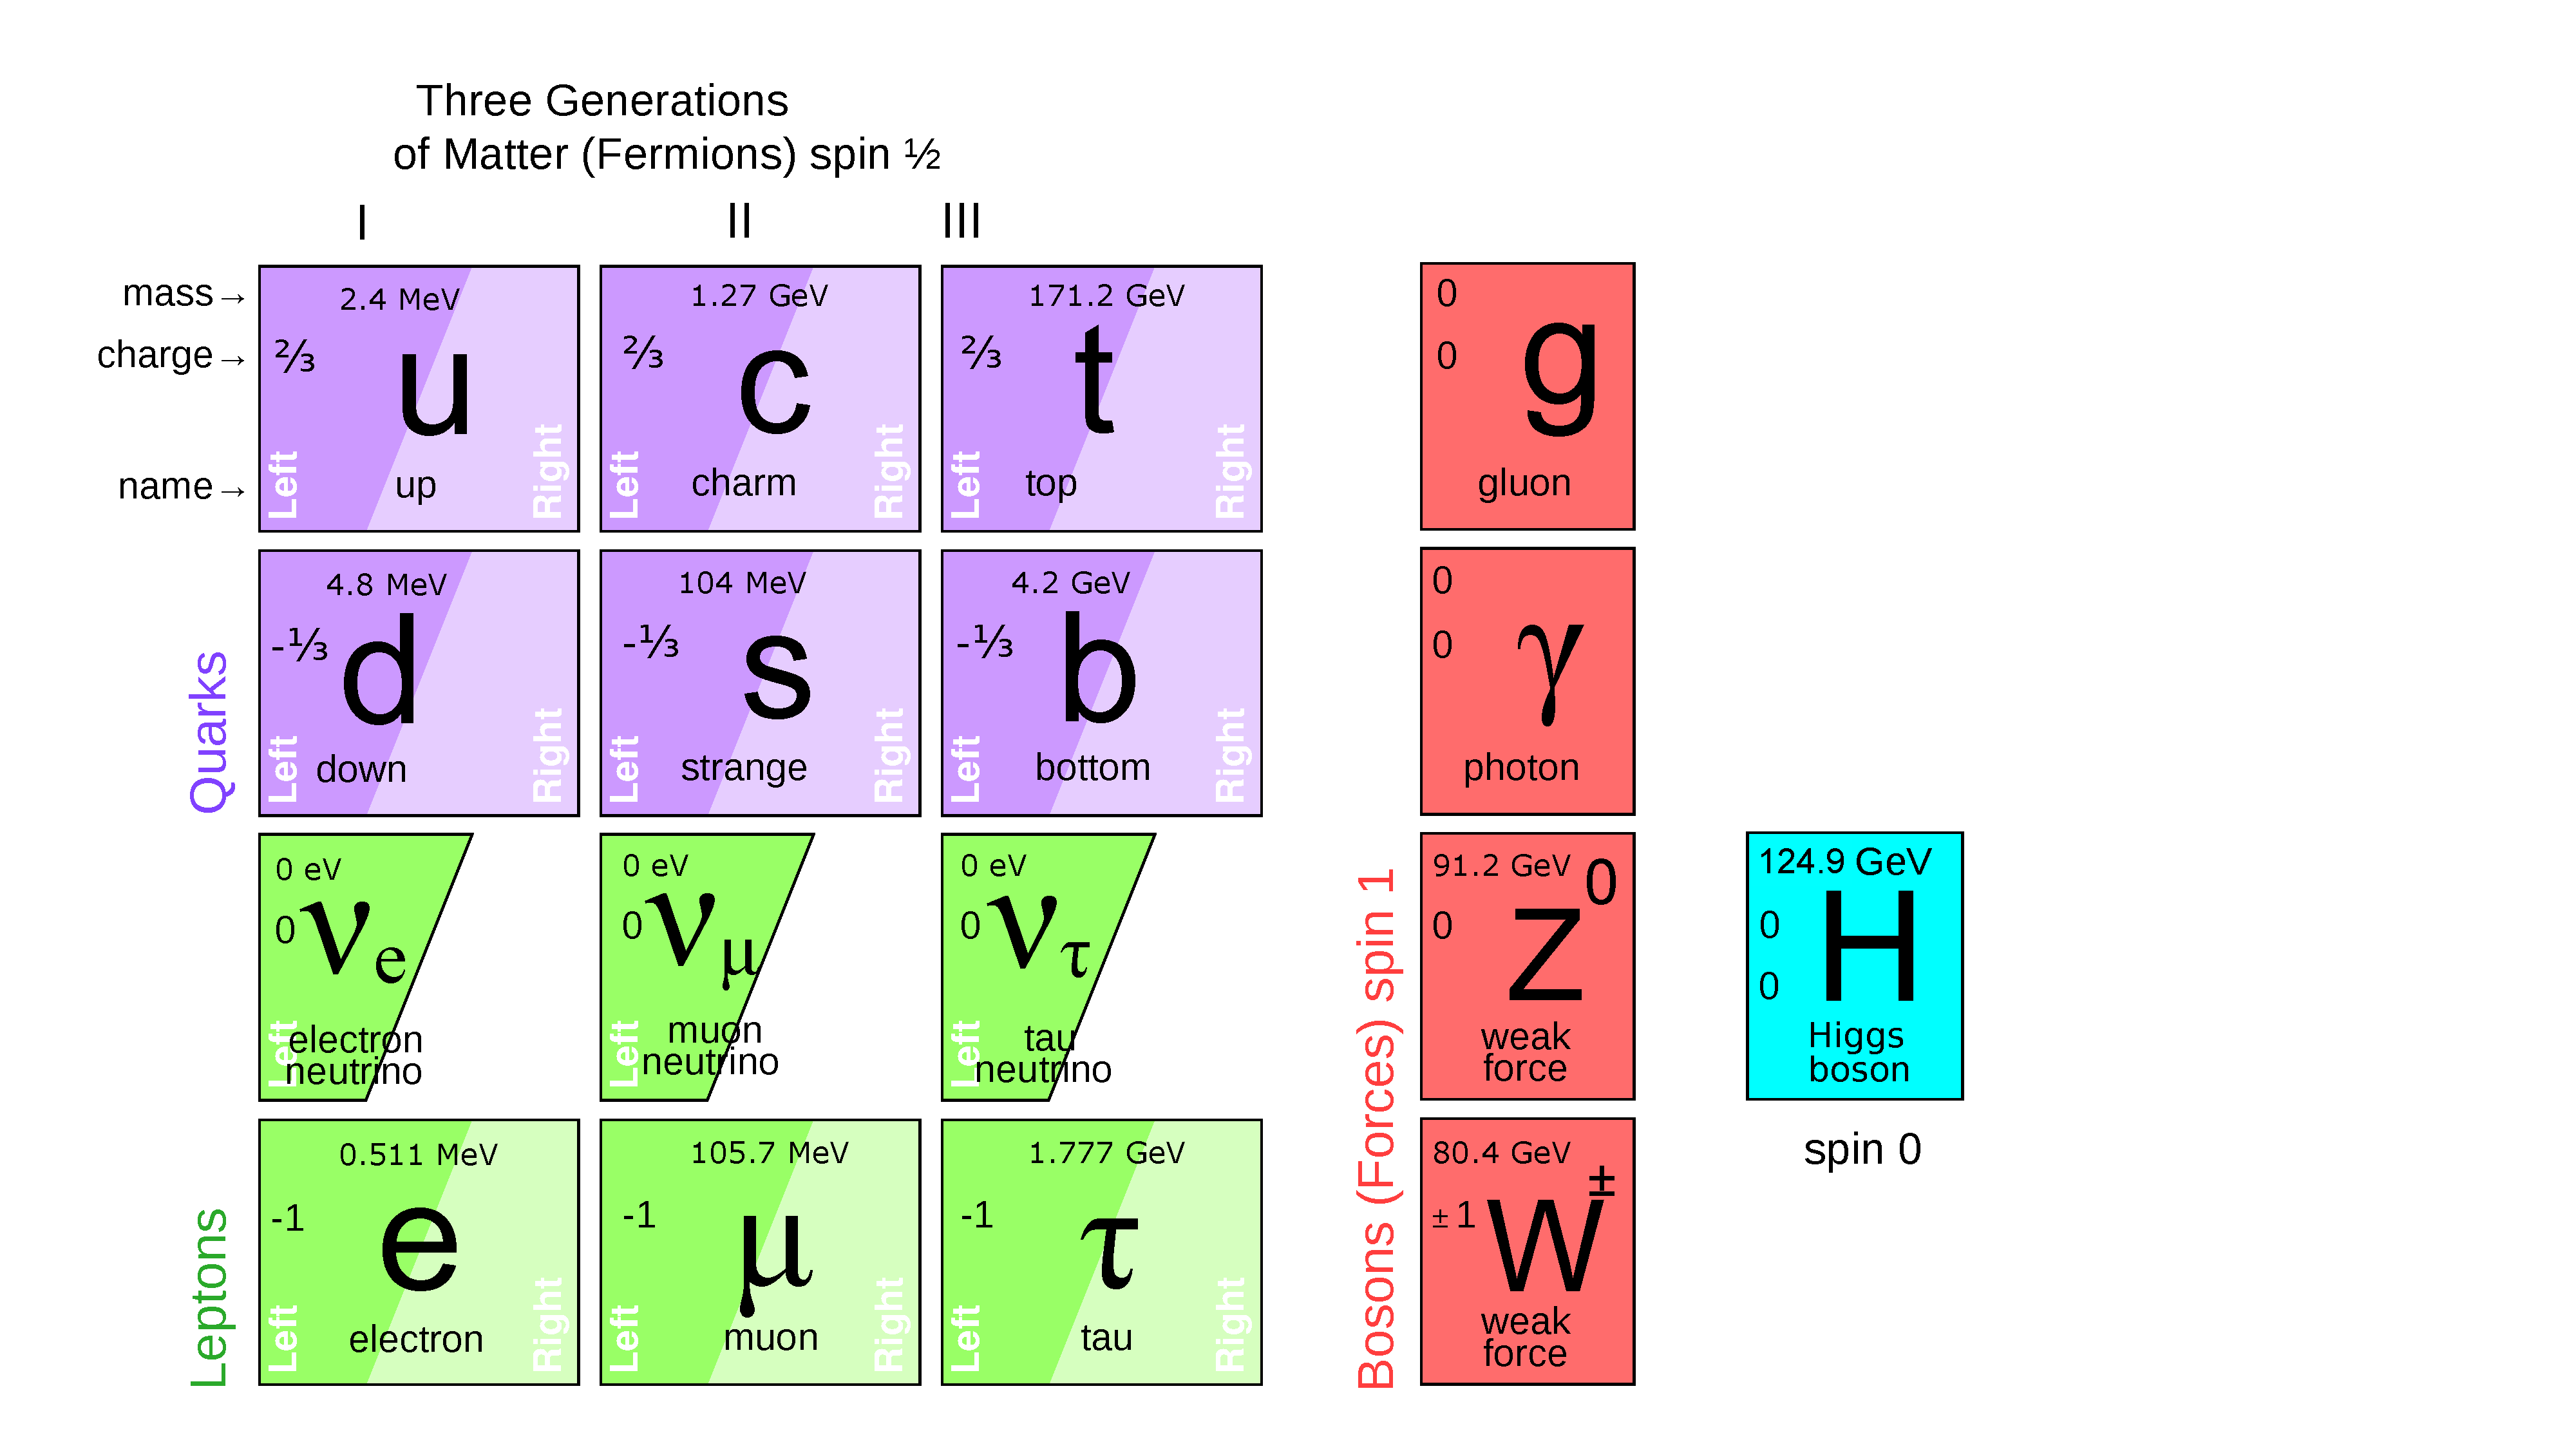
\includegraphics[width=.8\linewidth]{figures/theory/SM_no_HNL.pdf}
    \caption{The elementary particles in the Standard Model with their mass and electric charge.~\cite{Gninenko2012}}
    \label{fig:sm}
\end{figure}

The particles of the SM are summarized in~\cref{fig:sm} along with their mass and electric charge. The fermions are organized in three generations (two particles per generation) and two families. The first family is quarks, which have non-zero electric and color charges. Since these are quantum numbers for the EM and QCD interactions, quarks participate in both. The three generations of quarks are \textit{up}/\textit{down}, \textit{charm}/\textit{strange}, and \textit{top}/\textit{bottom}, commonly identified as quark flavors where the flavor is designated by the first letter of their names. The second family of fermions is leptons. Each generation of leptons consists a (electrically) charged-neutral pair, where the charged particles participate in the EM interaction while none of them participate in QCD. The charged leptons are \textit{electrons} ($e$), \textit{muons} ($\mu$), and \textit{taus} ($\tau$) each having a neutral partner \textit{neutrino} ($\nu_e,\,\nu_\mu,\,\nu_\tau$). Each fermion has an anti-fermion partner with an indentical mass and magnitude of spin but opposite physical charges. All fermions have non-zero weak isospin quantum numbers (with the caveat of chirality, which is discussed later) and hence participate in the weak interaction. Due to color confinement\footnote{Gluons themselves have color charges (unlike photons and weak bosons which are not colored in their interactions), which makes the strong interaction a long range force and makes color neutral composite quark states energetically feasible. Increasing the separation between quarks allows for the creation of $q\bar{q}$ pairs, which are also color neutral.}, isolated quarks are not found in nature and instead form color-neutral bound states, called hadrons. Hadrons are typically bound states of two or three quarks (although unstable higher quark multiplicity bound states have also been observed~\cite{PhysRevLett.112.222002, PhysRevLett.131.031901}). Hadrons with two quarks (quark-anti-quark pair) are called mesons, for example pions ($\pi^+$ is a $u\bar{d}$ bound state), and hadrons with three quarks are called baryons, for example protons ($uud$) and neutrons ($udd$). 

The last and the most recently discovered piece of the SM is the scalar Higgs boson ($H$). The Higgs field gives mass to all massive fermions and gauge bosons.


\subsection{Mathematical Structure}
The Standard Model is a mass dimension-4 relativistic quantum field theory with nineteen free parameters. It is defined by the local $SU(3)_C \times SU(2)_L \times U(1)_Y$ gauge symmetry. (Roughly,) the three factors of the gauge symmetry give rise to the three fundamental interactions. The first of these is the $SU(3)_C$ gauge symmetry of QCD, where the $C$ stands for color, the quantum number of QCD. The $SU(2)_L \times U(1)_Y$ is the gauge symmetry followed in the EW theory, where the $L$ stands for left-handed, and $Y$ denotes the weak hypercharge, which related to the electric charge $Q$ and the third component of isospin $I_3$ as $Y=Q-I_3$, the quantum numbers of electroweak interaction. 

The quantum states of the fermionic fields are denoted by $\psi$, which are bi-spinors. They obey the Dirac equation in the Clifford algebra defined using a representation of four $4\times4$ matrices, called gamma ($\gamma$) matrices which follow the anti-commutation relation 
\begin{equation}
    \{\gamma^\mu, \gamma^\nu\}=2\eta^{\mu\nu}I_4,
\end{equation}
where $\eta_{\mu\nu}$ is the Minkowski metric and $I_4$ is the $4\times4$ unit matrix. Handedness refers to the chiral states of fermions extracted using the projection operator:
\begin{equation}
    \psi_L=\frac{1}{2}(1-\gamma^5)\psi,\,\, \psi_R=\frac{1}{2}(1+\gamma^5)\psi.
\end{equation}
$\psi_{L(R)}$ is called the left-(right-)handed component of $\psi$, and $\gamma^5\equiv i\gamma^0\gamma^1\gamma^2\gamma^3$ is the fifth gamma matrix. Chirality is a Lorentz-invariant quantity but not a constant of motion, meaning that a pure left-handed state can gain a right-handed component during flight, and vice versa. The left-handed fermions of the same generation form a doublet of the $SU(2)_L$ symmetry. The quark doublets are represented as $Q_L\equiv (u_L\,\, d_L)^T$ and the lepton doublets are represented as $L_L \equiv (\nu_{e,L}\,\, e_L)^T$, with similar definitions for all three generations. The right-handed quarks, such as $u_R$ and $d_R$, and the right-handed charged leptons, such as $e_R$, are singlets of the $SU(2)_L$ symmetry whereas the right-handed neutrinos, $\nu_R$, would not have charges under any interaction. Right-handed neutrinos have not been observed in nature from direct or indirect measurements, and are not part of the SM. Right-handed fermion particles (and left-handed anti-particles) have a third component of weakisospin $I_3=0$, and hence do not participate in the weak interaction.~\Cref{tab:fermion_charges} summarizes the electric charge, weak hypercharge, and the third component of the weak isospin for the fermionic fields.

\begin{table}[!htbp]
    \centering
    \begin{tabular}{cccc}
    \hline \hline
         Field & $Q$ & $I_3$ & $Y=Q-I_3$ \\
         \hline
         \multirow{2}{*}{$Q_L = \left(\begin{array}{c} u_L \\ d_L \end{array}\right)$} & +2/3 & +1/2 & \multirow{2}{*}{1/6} \\
         & -1/3 & -1/2 & \\
         $u_R$ & +2/3 & 0 & +2/3 \\
         $d_R$ & -1/3 & 0 & -1/3 \\
         \hline
         \multirow{2}{*}{$L_L = \left(\begin{array}{c} \nu_{e,L} \\ e_L \end{array}\right)$} & 0 & +1/2 & \multirow{2}{*}{-1/2} \\
         & -1 & -1/2 & \\
         $e_R$ & -1 & 0 & -1 \\
         \hline\hline
    \end{tabular}
    \caption{The Standard Model fermion fields and their electric charge $Q$, third component of isospin $I_3$, and the weak hypercharge $Y$.}
    \label{tab:fermion_charges}
\end{table}

The $SU(3)_C$, $SU(2)_L$, and $U(1)_Y$ gauge fields are denoted by $G_\mu^a$ ($a=1,...,8$), $W_\mu^b$ ($b=1,\,2,\,3$), and $B_\mu$, respectively. Lastly, the Higgs field $\Phi$ is a complex scalar doublet of $SU(2)_L$. The Lagrangian of the Standard Model is given by:
\begin{equation}
\begin{split}    
    \mathcal{L}_{\mathrm{SM}}\equiv &
    \underbrace{-\frac{1}{4}G_{\mu\nu}^a G^{\mu\nu}_a-\frac{1}{4}W_{\mu\nu}^b W^{\mu\nu}_b-\frac{1}{4}B_{\mu\nu}B^{\mu\nu}}_\text{gauge term}+
    \underbrace{\vphantom{\frac{.}{.}}i \bar{\psi} \gamma^\mu D_\mu \psi}_\text{kinetic term}+ \\
    & \underbrace{\vphantom{\frac{.}{.}}\bar{\psi_i} y_{i j} \psi_j \Phi+h.c.}_\text{Yukawa term}+
    \underbrace{\vphantom{\frac{.}{.}}\left|D_\mu \Phi\right|^2}_\text{Higgs-gauge coupling}-
    \underbrace{\vphantom{\frac{.}{.}}V(\Phi)}_\text{Higgs potential}
    ,
\end{split}
\end{equation}
where $G_{\mu\nu}^a$, $W_{\mu\nu}^b$, and $B_{\mu\nu}$ represent the field strength tensors of strong, weak isospin, and weak hypercharge fields, and $h.c.$ stands for the hermitian conjugate of the previous term. For simplicity, the sum over the fermionic fields in not shown, and the Yukawa term is also simplified. The field strength tensor for a field $V$ is given by
\begin{equation}
    V_{\mu\nu}^i \equiv \partial_\mu V_\nu^i - \partial_\nu V_\mu^i + g_V f_{ijk} V_\mu^jV_\nu^k,
\end{equation}
where $i$, $j$, and $k$ are indices corresponding to the number of fields for a force, $g_V$ is the coupling constant for the field, and $f_{ijk}$ is the structure constant for the symmetry group. The kinetic terms consists of the covariant derivative $D_\mu$, defined as
\begin{equation}
    D_\mu \equiv \partial_\mu - i g_s\frac{1}{2}\Sigma_a\lambda^a G_\mu^a -i g \frac{1}{2}\Sigma_b\sigma^b W_\mu^b -i g' Y B_\mu, 
\end{equation}
where $g_s$, $g$, and $g'$ are the coupling constants of the strong, weak isospin, and weak hypercharge fields, respectively, $\lambda$ are the Gell-Mann matrices, and $\sigma$ are the Pauli matrices which form a representation of the respective symmetry groups.

The Higgs mechanism~\cite{PhysRevLett.13.508, PhysRevLett.13.321} is responsible for spontaneous breaking of the EW symmetry, which ascribes masses to three of the four gauge bosons and leaves the photon massless. At low energies, the Higgs field acquires a non-zero vacuum expectation value ($v$) and orients itself along an (arbitrary) direction in the field space. The direction is normally chosen to minimize degrees of freedom, and the Higgs doublet becomes
\begin{equation}\label{eq:higgs_vev}
    \Phi = \frac{1}{\sqrt{2}}\left(\begin{array}{c} 0 \\ v+h \end{array}\right),
\end{equation}
where $h$ is an excitation of the Higgs scalar field. The masses of the gauge bosons (or rather of their mass eigenstates) become
\begin{equation}
\begin{split}
m_\gamma &= 0, \\
m_Z &= \frac{v}{2}\sqrt{g^2 + g'^2}, \text{ and} \\
m_{W^\pm} &=  \frac{gv}{2}.
\end{split}
\end{equation}
After the EW symmetry is broken, the Yukawa term decomposes into two terms: an interaction term between the fermions and the Higgs scalar, the strength of which is proportional to the fermion mass, and a Dirac mass term for all (massive) fermions, which is of the form
\begin{equation}
    \mathcal{L_\text{Dirac mass}} = -m (\bar{\psi}_L\psi_R + \bar{\psi}_R\psi_L).
\end{equation}
Since $\nu_R$ do not exist within the SM, no such higgs interaction term mass term exists for neutrinos, causing them to be massless.

\subsection{Limitations of Standard Model}
The Standard Model has survived the test of time and has proved to be the most well-tested theory of natural phenomena. It has enjoyed incredible success in making predictions validated by highly precise measurements, such as the 16 parts-per-trillion validation of the CPT invariance of the Standard Model by the BASE experiment~\cite{Borchert2022}, less than 1 parts-per-trillion test of the electron magnetic moment~\cite{PhysRevA.83.052122}, the 0.2 parts-per-mil measurement of the $W$-boson mass~\cite{atlascollaboration2024measurement} and the measurements of Higgs boson properties by the ATLAS~\cite{ATLASNature} and CMS~\cite{CMSNature} experiments.

However, quite a few open problems with experimental evidences taint this success. One such problem is that of matter-anti-matter asymmetry, which questions the theoretical basis of the large ratio of matter to anti-matter in the universe. The SM provides no mechanism/reason for this asymmetry coming from interactions in the early univerise. Many astronomical measurements, such as that of the rotational curves of spiral galaxies~\cite{Begeman:1989kf}, prove the existence of an invisible kind of matter, called \textit{dark matter}, that forms a larger portion of the universe's energy density than the visible matter predicted in the SM. None of the SM particles can act as dark matter, which poses a question about its particulate nature. The observation most relevant to this thesis and the only direct observation of a BSM phenomena is that of neutrino flavor oscillations. Neutrinos of a specific flavor propagating through space can convert into a different flavor. Such oscillations have been observed in solar neutrinos~\cite{PhysRevLett.87.071301}, atmospheric atmospheric neutrinos~\cite{PhysRevLett.81.1562}, reactor neutrinos~\cite{PhysRevLett.108.171803}, as well as in neutrino beams~\cite{PhysRevD.88.032002}. Neutrino oscillations can be explained by neutrino mass eigenstates. The Pontecorvo–Maki–Nakagawa–Sakata (PMNS) matrix~\cite{Maki1962} parameterizes the mixing between neutrino flavor and mass eigenstates. In this framework, the probability of observing a different neutrino flavor than what was originally produced is found to be proportional to the difference of square of masses of neutrino mass eigenstates. The oscillations have been studied in detail, and independent measurements of the PMNS matrix elements have been found to be consistent with each other. Since neutrinos are massless in the SM, these observations strongly suggests a BSM effect giving rise to neutrino masses.

\section{Heavy Neutral Leptons}\label{sec:hnl}

Right-handed massive neutrinos are proposed in a large number of BSM extensions in an attempt to provide a complete theory of the universe. They are often referred to as \textit{sterile} neutrinos since they do not engage in any of the gauge interactions. Heavy Neutral Leptons are a similar class of particles that typically contain a superposition of left- and right-handed components and are characterized by the square of couplings (or mixing angles) to SM neutrinos ($|U_e|^2$, $|U_\mu|^2$, and $|U_\tau|^2$). Historically, right-handed neutrinos were introduced as parts of larger gauge groups~\cite{PhysRevD.11.2558} driven by general principles, such as unified theories~\cite{PhysRevD.10.275}, to introduce a seesaw mechanism for neutrino masses. A type-I seesaw mechanism provided by HNLs can also explain neutrino masses at the eV scale~\cite{PhysRevD.22.2227}. The simplest renormalizable extension to the SM consistent with neutrino oscillation measurements adds $\mathcal{N}(\geq 2)$ right-handed $SU(2)_L\times U(1)_Y$ singlet neutrinos. Such minimal extensions are not only adept at explaining neutrino masses, but also offer solutions to other open problems in particle physics such as the baryon-asymmetry in the universe, which can be explained using $\mathcal{N}=2$ models via leptogenesis~\cite{Kuzmin1985}. For example, for HNL Majorana masses of the order of the electroweak scale or below, the seesaw mechanism imposes the HNL Yukawa couplings to be small to make the active neutrino masses consistent with flavor oscillation results. The production of HNLs followed by their charge parity-violating decays in the early universe can explain this matter-antimatter asymmetry.~\cite{Asaka2005, Fukugita1986}. The addition of a light HNL with a very small Yukawa coupling can also provide a dark matter candidate~\cite{PhysRevLett.72.17, Asaka2005}. The rather simple structure of HNL-incorporating models and their versatile use to explain BSM phenomena make their searches very attractive.

\subsection{Standard Model Extension}
The description of the mechanism of generation of neutrino masses via a neutrino portal has been adapted from~\cite{Alekhin2016}. The Lagrangian for a minimal extension of the SM, $\mathcal{L_\mathrm{SM+HNL}}$, by $\mathcal{N}$ right-handed HNLs $N_I$ is given by:
\begin{equation}\label{eq:sm_extension}
    \mathcal{L_\mathrm{SM+HNL}}-\mathcal{L_\mathrm{SM}}=\mathcal{L}'= 
    i\bar{N_I}\gamma^\mu \partial_\mu N_I - \left( F_{\alpha I}\bar{L}_{L\alpha}N_I\tilde{\Phi} + \frac{M_I}{2}\bar{N_I^C} N_I + h.c.  \right),
\end{equation}
where $I=1,...,\mathcal{N}$. $\alpha$ is the lepton flavor index running over $\{e, \mu, \tau\}$; $F_{\alpha I}$ is the Yukawa coupling between the $\alpha$ left-handed doublet and $N_I$; $L_L$ is the left-handed lepton doublet $(\nu_L,\,\,e_L)^T$; $\tilde{\Phi}=i\sigma_2\Phi$; $M_I$ is the mass of $N_I$; and $N^C_I$ is the charge conjugated state of $N_I$. The extension consists of a kinetic term, the Yukawa term, and a Majorana mass term, $-\frac{M_I}{2}\bar{N_I^C} N_I$, which is allowed since $N_I$ are not charged under any gauge transformations. The SM extension for $\mathcal{N}=3$ is illustrated ~\cref{fig:sm_extended}.

\begin{figure}[!th]
    \centering
    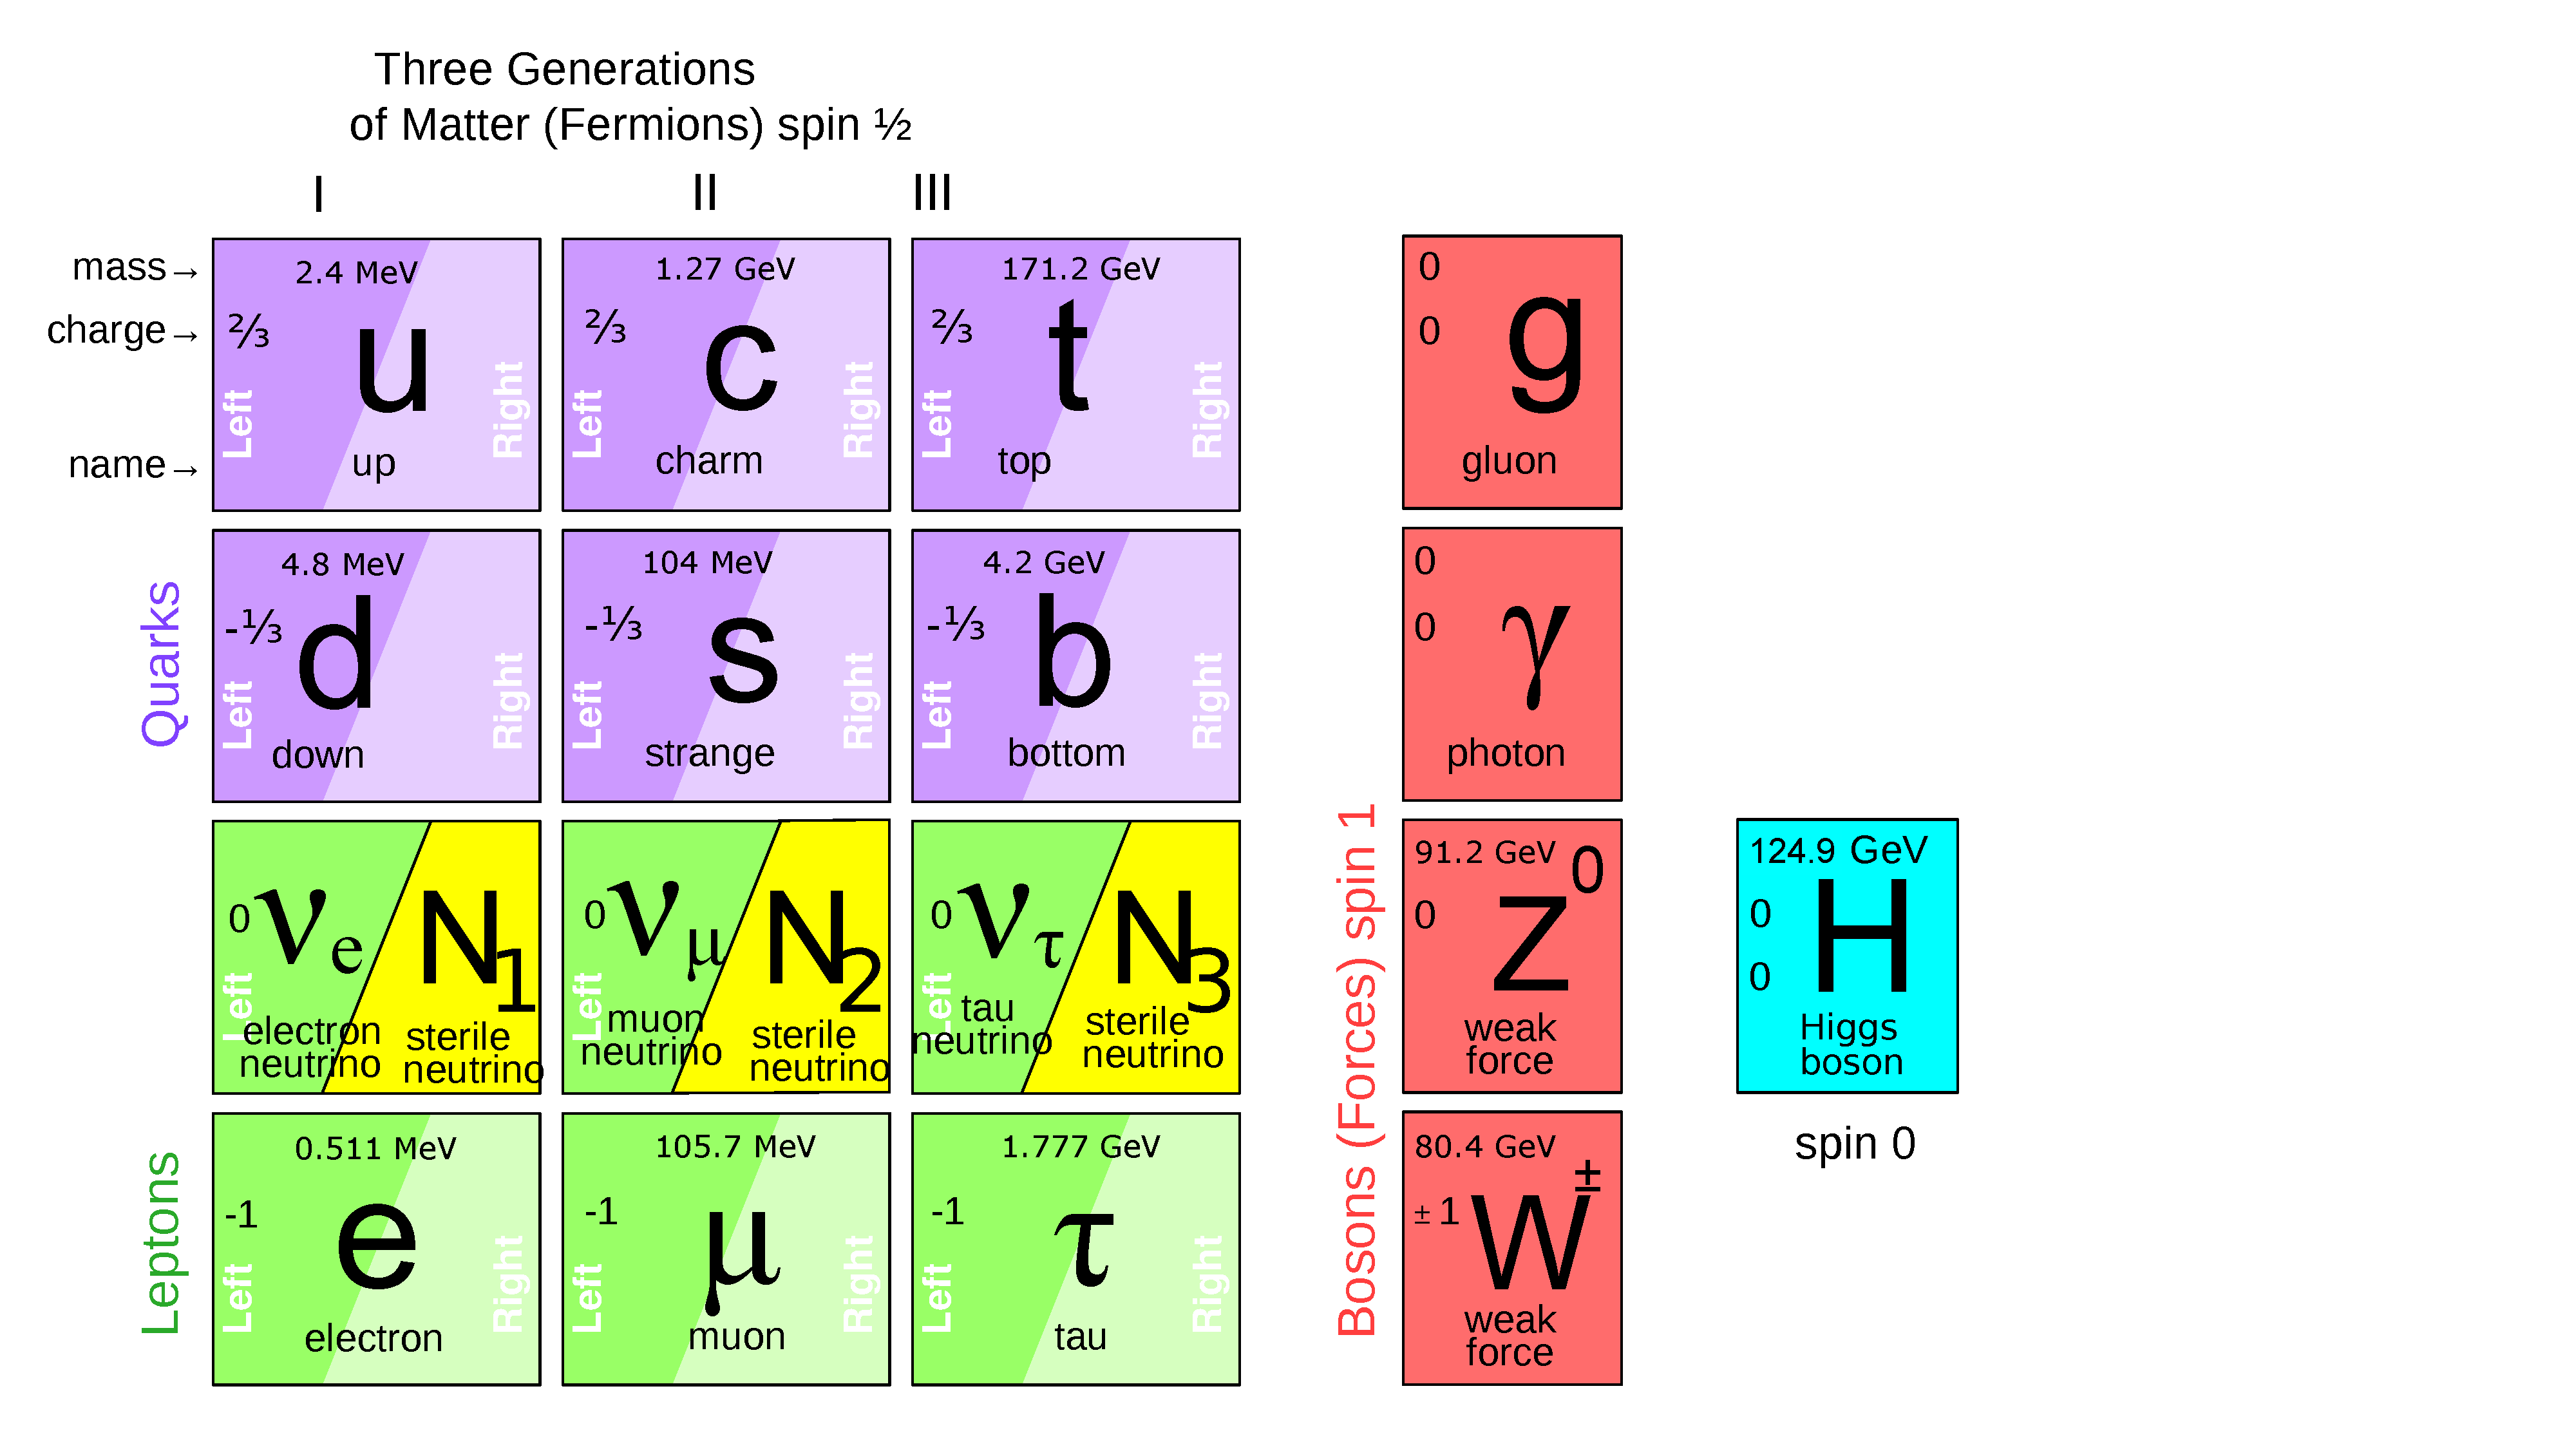
\includegraphics[width=.8\linewidth]{figures/theory/SM_with_HNL.pdf}
    \caption{The elementary particles in the Standard Model along with $\mathcal{N}=3$ right-handed Majorana neutrinos.~\cite{Gninenko2012}}
    \label{fig:sm_extended}
\end{figure}

At low energies, the Higgs field acquires a non-zero $v$ as shown in~\cref{eq:higgs_vev}, and~\cref{eq:sm_extension} can be written as:
\begin{equation}
    \mathcal{L}'=\mathcal{L}_\mathrm{kinetic}+\mathcal{L}_\mathrm{Majorana}-vF_{\alpha I}\bar{\nu}_{L\alpha}N_I - \frac{F_{\alpha I}}{\sqrt{2}}\bar{\nu}_{L\alpha}N_I h.
\end{equation}

Thus, a Dirac mass term $-vF_{\alpha I}\bar{\nu}_{L\alpha}N_I$ is generated which allows for $\nu_\alpha - N_I$ mixing. The charge eigenstates of~\cref{eq:sm_extension} do not coincide with the mass eigenstates, where the latter can be obtained by diagonalizing the mass-matrix. In the limit $vF_{\alpha I} \ll M_I$, the active neutrino masses (3 eigenvalues) become much smaller than $M_I$ (other $\mathcal{N}$ eigenvalues, up to a small admixture of $\nu_\alpha$) and the electroweak scale $v$. The smallness of the left-handed admixture in the mass eigenstates is characterized by the ratio of the Dirac and Majorana masses,
\begin{equation}\label{eq:mixing}
    |\Theta_{\alpha I}|^2=\frac{v^2|F_{\alpha I}|}{M_I^2} \ll 1,
\end{equation}
where $\Theta_{\alpha I}$ is the mixing angle between left-handed neutrino flavor $\alpha$ and right-handed HNL $N_I$. This is known as the seesaw mechanism, since a larger HNL mass in comparison to the Dirac mass leads to a lower active mass eigenvalue.

The six free parameters of the PMNS matrix\footnote{Typically, the PMNS matrix is defined with four free parameters consisting of three mixing angles and one charge-parity violating phase. Such a parameterization assumes a Dirac neutrino. For Majorana neutrinos, two additional phases are included for a total of six free parameters.} and the three active mass eigenvalues add a total of nine extra parameters to the SM. To accommodate these parameters, $\mathcal{N}\geq 2$ HNLs are required in a valid SM extension. The search presented in this thesis considers two approaches to search for HNLs. A model-independent approach is presented where only a single HNL is kinematically accessible with any other HNLs expected to be beyond the mass scales probed by the analysis. Two single-flavor mixing (1SFH) scenarios are considered in this approach, first where the accessible HNL only mixes with $\nu_\mu$ (1SFH($\mu$)) and second only with $\nu_e$ (1SFH($e$)). A model-dependent approach is also presented, where the results are interpreted in a two-quasi degenerate model (2QDH)~\cite{Tastet2021}. This model considers two HNLs with nearly degenerate masses ($M_1\sim M_2$, $m_\mathrm{HNL}=\frac{M_1+M_2}{2}$), where $|M_1-M_2|$ is smaller than the detector resolution. The four models considered are tabulated in~\cref{tab:hnl_models}.

HNLs in this analysis refer to the states corresponding to large(r) mass eigenvalues, which consist mainly of the right-handed heavy neutrino $N_I$ and a small admixture of left-handed neutrinos allowing it to participate in the weak interaction. The strength of this interaction is governed by the mixing angles. The experimentally relevant observable measured in this analysis is given by:
\begin{equation}
    |U_\alpha|^2 \equiv \Sigma_{I=1}^{\mathcal{N}} |\Theta_{\alpha I}|^2,
\end{equation}
where $\alpha={e,\mu,\tau}$. $|U_\alpha|$ is the coupling, or the strength of interaction, between an HNL to a SM neutrino of the flavor $\alpha$. The total square of coupling strength of HNLs with the SM neutrinos is:
\begin{equation}
    |U|^2 \equiv \Sigma_\alpha |U_\alpha|^2 = \Sigma_{\alpha,I}|\Theta_{\alpha I}|^2.
\end{equation}

Since the mixing angles $\Theta_{\alpha I}$ are related to the Yukawa couplings $F_{\alpha I}$ as shown in~\cref{eq:mixing}, the current limits on these Yukawa couplings obtained using neutrino oscillation data can be used to impose constraints on $|U_\alpha|$ as well. NuFIT provides an updated global analysis of neutrino mixing data~\cite{Esteban2020}, which was further analysed in~\cite{Tastet2021} to obtain the corresponding limits on relative mixing angles of HNLs with the three different neutrino flavors, $x_\alpha = |U_\alpha|^2 / |U|^2$. The neutrino oscillation data offers two possibilities on the ordering of active neutrino masses:
\begin{itemize}
    \item Normal Hierarchy (NH): $m_1 < m_2 < m_3$ i.e. $\Delta m_{31}^2 > 0$, and
    \item Inverted Hierarchy (IH): $m_3 < m_1 < m_2$ i.e. $\Delta m_{31}^2 < 0$.
\end{itemize}

\begin{figure}[!htb]
    \centering
    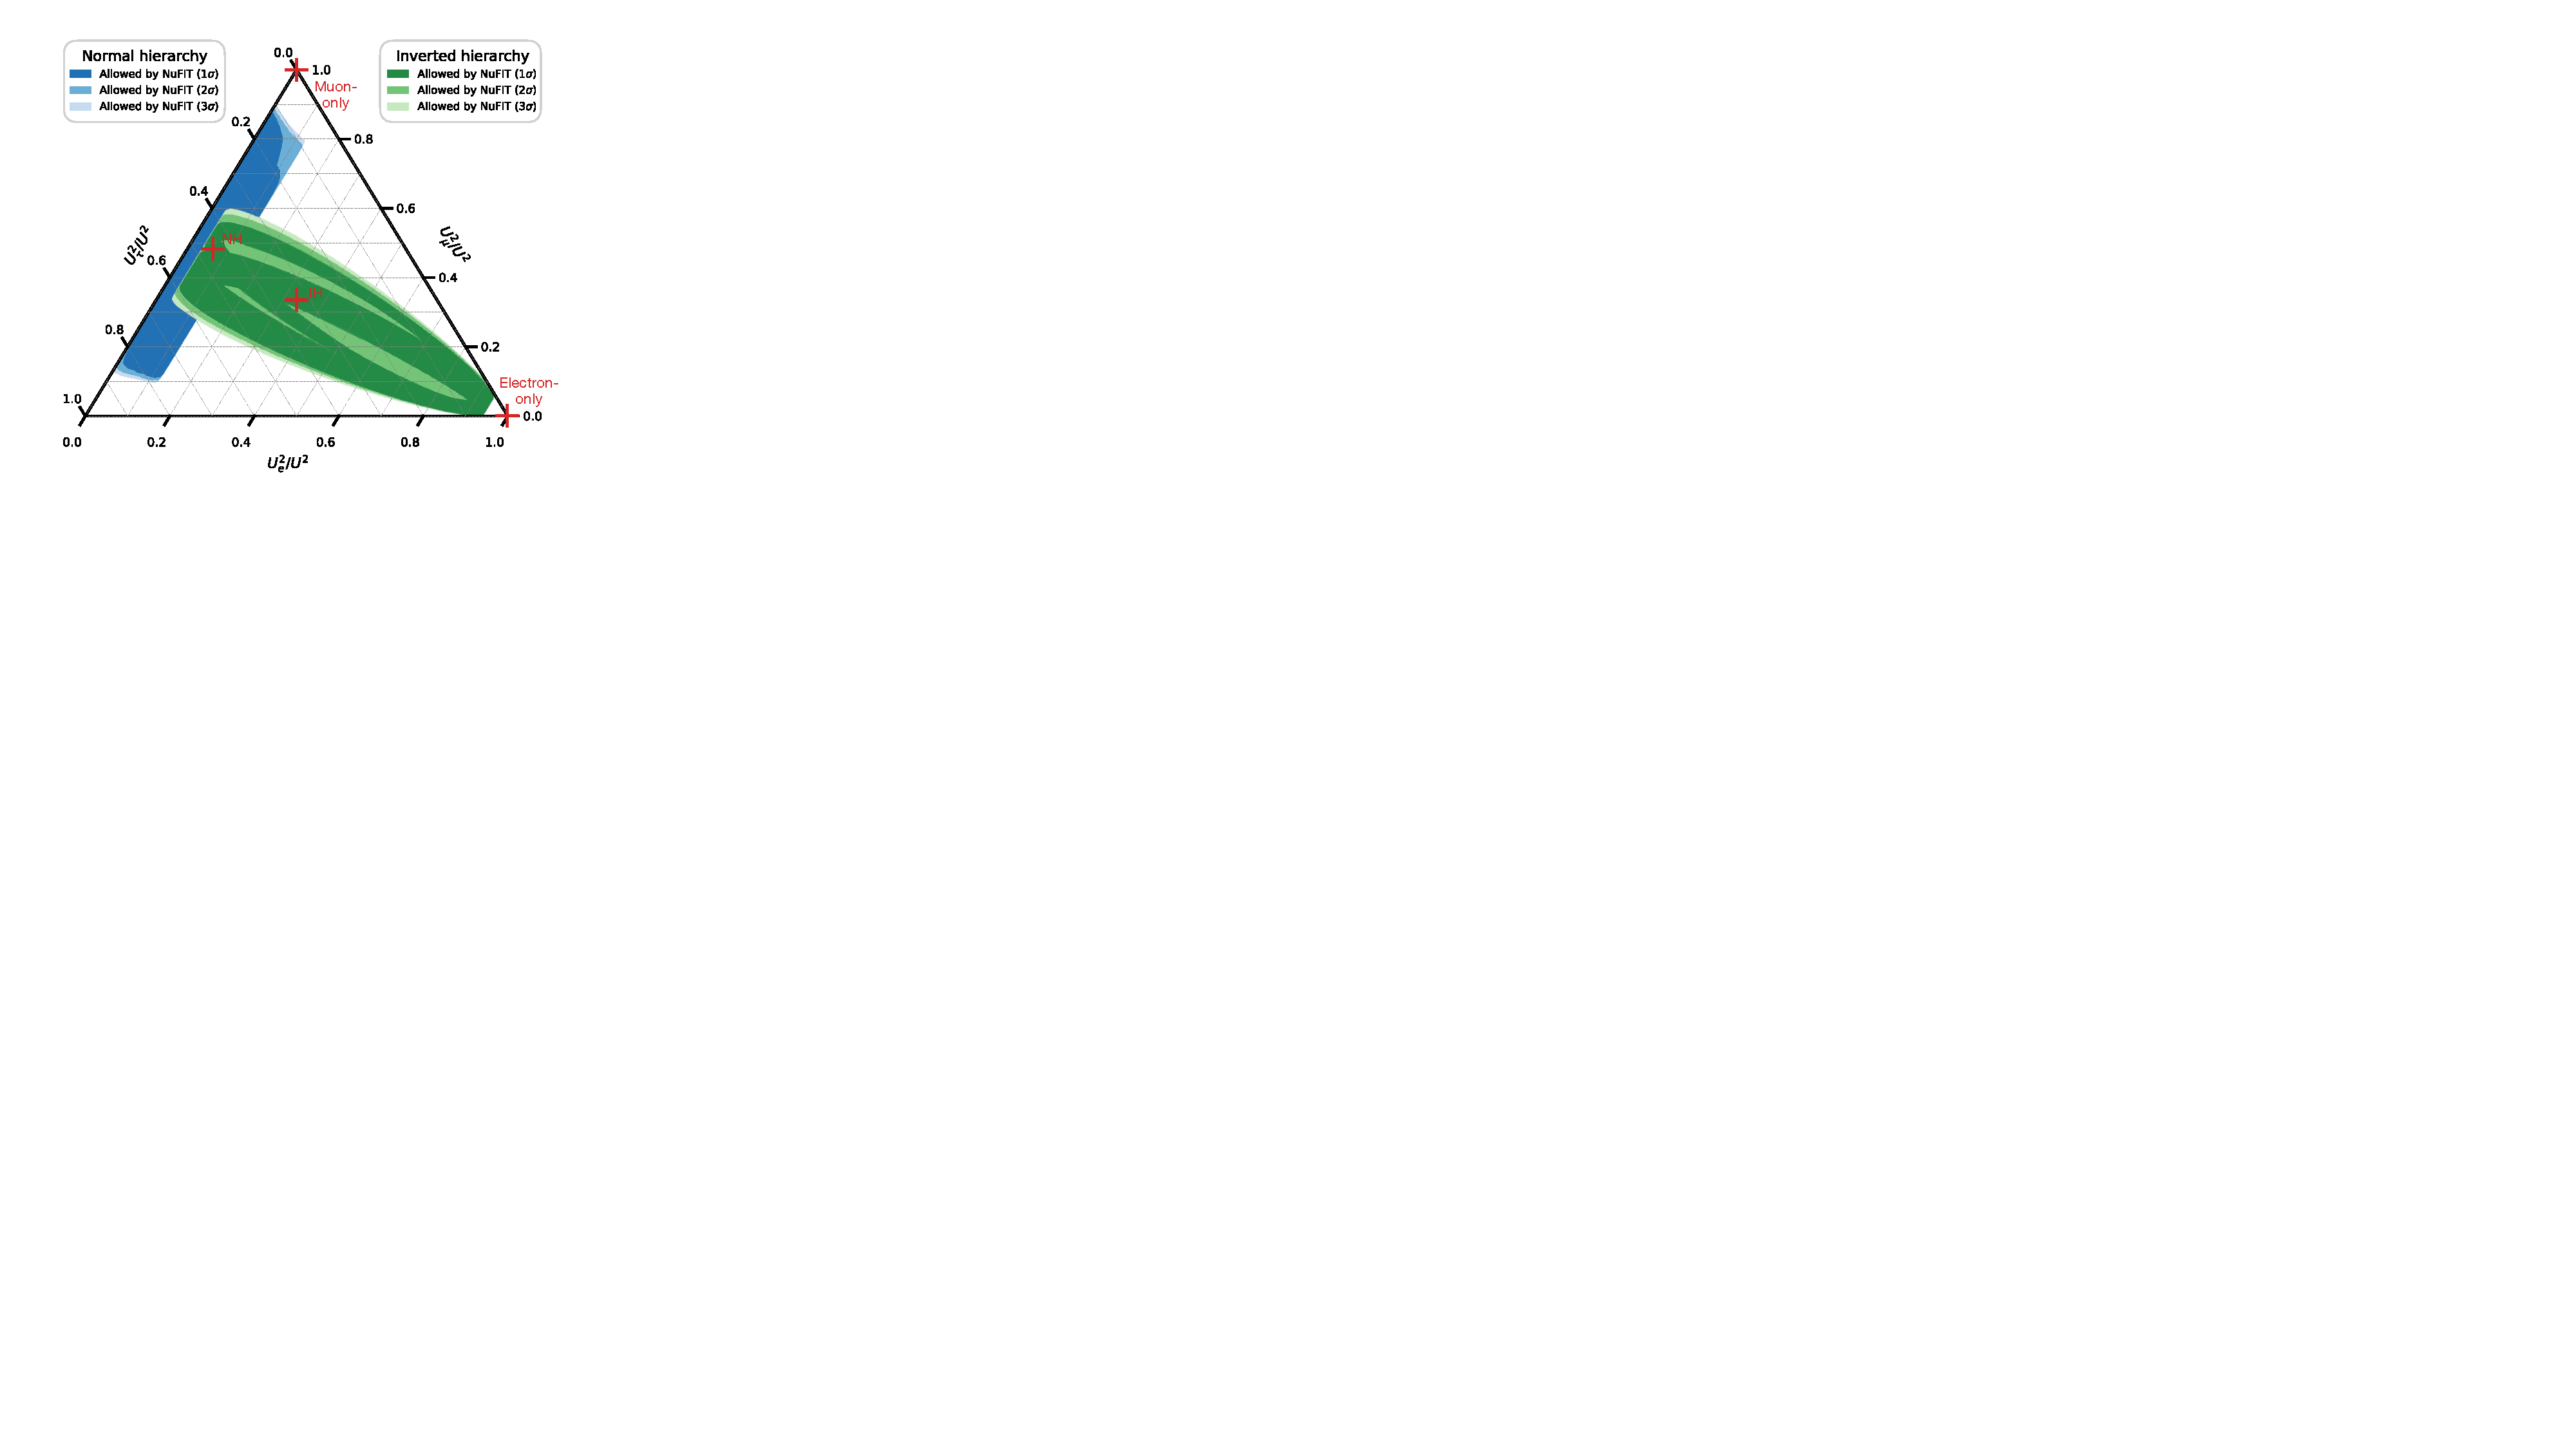
\includegraphics[width=.6\linewidth]{figures/theory/Jean_Loup_IH_NH_diagram.pdf}
    \caption{Allowed combinations of $x_\alpha = |U_\alpha|^2 / |U|^2$ consistent with recent neutrino oscillation data. The combinations allowed by a normal mass ordering is shown in blue and those allowed by an inverted mass ordering are shown in green. The red crosses represent the benchmark scenarios probed in this analysis. Figure adapted from~\cite{Tastet2021}.}
    \label{fig:IH_NH_diagram}
\end{figure}

~\Cref{fig:IH_NH_diagram} shows the allowed combinations of $x_\alpha$ consistent with neutrino oscillation data. The 2QDH model considered in this analysis is interpreted in an IH and a NH mixing scenario. Typically, most experiments report limits on HNL-$\nu$ couplings in a single-flavor mixing scenarios which are more simplistic and hence allow for direct comparisons with other results. Hence, two model-independent 1SFH($\mu$) and 1SFH($e$) scenarios are considered as well. Since $\tau$-leptons are unstable and decay rapidly, they are below the acceptance level of the analysis, and hence a mixing to them is not considered. The four scenarios probed in this analysis are identified with red crosses in~\cref{fig:IH_NH_diagram}.~\Cref{tab:hnl_models} shows the combinations $x_\alpha$ used for the four benchmark models used in this analysis.


\begin{table}[!htbp]
    \centering
    \begin{tabular}{cccc}
    \hline\hline
        Model & $x_e$ & $x_\mu$ & $x_\tau$ \\
        \hline
        1SFH($e$) & 1 & 0 & 0 \\
        1SFH($\mu$) & 0 & 1 & 0 \\
        2QDH(IH) & 1/3 & 1/3 & 1/3 \\
        2QDH(NH) & 0.06 & 0.48 & 0.46 \\
        \hline
    \end{tabular}
    \caption{Relative mixing $x_\alpha = |U_\alpha|^2 / |U|^2$ for the four benchmark models used in this analysis.}
    \label{tab:hnl_models}
\end{table}

\subsection{HNL Production and Decay}
This analysis searches for an HNL produced in decays of the $W$-boson via the $W\to \ell_\alpha N$ mechanism. The HNL production cross-section $\sigma_N$ depends on the rate of production of the $W$ boson in proton--proton collisions and the branching ratio of $W\to \ell_\alpha N$:
\begin{equation}
    \sigma_N = \sigma(pp\to W) \cdot BR(W\to \ell_\alpha N).
\end{equation}
The branching ratio depends on the mass of the HNL (\mhnl), the HNL-$\nu_\alpha$ couplings, and the SM branching ratio of $W\to \ell_\alpha \nu_\alpha$, since only the left-handed admixture participates in the weak interaction:
\begin{equation}
     \sigma_N = x_\alpha |U|^2 \cdot \sigma(pp\to W) \cdot BR(W\to \ell_\alpha \nu_\alpha) \left( 1-\frac{\mhnl^2}{m_W^2} \right)^2 \left( 1+\frac{\mhnl^2}{m_W^2} \right).
\end{equation}

For the 2QDH model, the production cross-section effectively doubles since the contribution from two HNLs adds up instead of a one single-flavor mixing HNL.

The final state probed in this analysis are the leptonic decays of the HNL ($N \to \ell_\beta \ell_\gamma \nu$), as shown in~\cref{fig:feynman}. If the charged leptons in the decay are of the same flavor, both charged and neutral currents contribute to the decay. Only decays of $W^+$ are shown for illustration, but both $W^+$-and $W^-$-initiated decays are considered in the analysis.

\begin{figure}[ht!]
\centering
\subfloat[Charged current decay]{
\resizebox{0.45\linewidth}{!}{
\begin{tikzpicture}[]
  \begin{feynman}
    \vertex (a) {\(W^{+}\)};
    \vertex [right=of a] (b);
    \vertex [above right=of b] (f1) {\(\ell_\alpha^{+}\)};
    \vertex [below right=of b] (c);
    \vertex [below right=of c] (f2) {\(\ell_\beta^{-}\)};
    \vertex[right=of c] (d);
    \vertex[above right=of d] (f3) {\(\ell_\gamma^{+}\)};
    \vertex[below right=of d] (f4) {\(\nu_{\gamma}\)};

    \diagram* {
      (a) -- [boson] 
      (b) -- [anti fermion] (f1),
      (b) -- [red, scalar, edge label'=\(N\)] (c),
      (c) -- [boson, edge label=\(W^{+\star}\)] (d),
      (c) -- [fermion] (f2),
      (d) -- [anti fermion] (f3),
      (d) -- [fermion] (f4),
    };
  \end{feynman}
\end{tikzpicture}
} }
\subfloat[Neutral current decay]{
\resizebox{0.45\linewidth}{!}{
\begin{tikzpicture}[]
  \begin{feynman}
    \vertex (a) {\(W^{+}\)};
    \vertex [right=of a] (b);
    \vertex [above right=of b] (f1) {\(\ell_\alpha^{+}\)};
    \vertex [below right=of b] (c);
    \vertex [below right=of c] (f2) {\(\nu_\beta\)};
    \vertex[right=of c] (d);
    \vertex[above right=of d] (f3) {\(\ell_\gamma^{+}\)};
    \vertex[below right=of d] (f4) {\(\ell_\gamma^{-}\)};

    \diagram* {
      (a) -- [boson] 
      (b) -- [anti fermion] (f1),
      (b) -- [red, scalar, edge label'=\(N\)] (c),
      (c) -- [boson, edge label=\(Z^{\star}\)] (d),
      (c) -- [fermion] (f2),
      (d) -- [anti fermion] (f3),
      (d) -- [fermion] (f4),
    };
  \end{feynman}
\end{tikzpicture}
} }
\caption{Feynman diagrams for the $W$ initiated HNL production and subsequent leptonic final state decay.}
\label{fig:feynman}
\end{figure}

The global $U(1)$ symmetry of the SM gives rise to an approximately conserved quantity during interactions, the total lepton number, given by number of leptons minus the number of anti-leptons. Since the HNLs probed in this analysis have Majorana mass terms in the extended SM Lagrangian, the particle and anti-particle states are identical. Hence, they can give rise to lepton number violating decays as well. Since there are no leptons in the initial state (proton--proton collisions are used), a lepton number conserving decay would lead to a net zero lepton number in the final state as well.~\Cref{fig:feynman_lnc_lnv} shows the Feynman diagrams for lepton number conserving and violating decays. An equal contribution from both decays are considered for all models.

\begin{figure}[ht!]
\centering
\subfloat[LNC]{
\resizebox{0.45\linewidth}{!}{
\begin{tikzpicture}[]
  \begin{feynman}
    \vertex (a) {\(W^{+}\)};
    \vertex [right=of a] (b);
    \vertex [above right=of b] (f1) {\(\ell_\alpha^{+}\)};
    \vertex [below right=of b] (c);
    \vertex [above right=of c] (f2) {\(\ell_\beta^{-}\)};
    \vertex[below right=of c] (d);
    \vertex[above right=of d] (f3) {\(\ell_\gamma^{+}\)};
    \vertex[below right=of d] (f4) {\(\nu_\gamma\)};

    \diagram* {
      (a) -- [boson] 
      (b) -- [anti fermion] (f1),
      (b) -- [red, scalar, edge label'=\(N\)] (c),
      (c) -- [boson, edge label=\(W^{+\star}\)] (d),
      (c) -- [fermion] (f2),
      (d) -- [anti fermion] (f3),
      (d) -- [fermion] (f4),
    };
  \end{feynman}
\end{tikzpicture}
} }
\subfloat[LNV]{
\resizebox{0.45\linewidth}{!}{
\begin{tikzpicture}[]
  \begin{feynman}
    \vertex (a) {\(W^{+}\)};
    \vertex [right=of a] (b);
    \vertex [above right=of b] (f1) {\(\ell_\alpha^{+}\)};
    \vertex [below right=of b] (c);
    \vertex [above right=of c] (f2) {\(\ell_\beta^{+}\)};
    \vertex[below right=of c] (d);
    \vertex[above right=of d] (f3) {\(\ell_\gamma^{-}\)};
    \vertex[below right=of d] (f4) {\(\bar{\nu_\gamma}\)};

    \diagram* {
      (a) -- [boson] 
      (b) -- [anti fermion] (f1),
      (b) -- [red, scalar, edge label'=\(N\)] (c),
      (c) -- [boson, edge label=\(W^{-\star}\)] (d),
      (c) -- [fermion] (f2),
      (d) -- [fermion] (f3),
      (d) -- [anti fermion] (f4),
    };
  \end{feynman}
\end{tikzpicture}
} }
\caption{Lepton number conserving (LNC) and lepton number violating (LNV) Feynman diagrams for the charged current HNL decay.}
\label{fig:feynman_lnc_lnv}
\end{figure}

The rate of observing an HNL decay in a specific final state is given by the product of its production cross-section and its branching ratio to a final state $BR(N\to \ell \ell \nu)$ where $\ell=e\text{ or }\mu$. The branching ratio depends on the possible charged and neutral current mediated decays and the coupling strength of the HNL to the different flavors SM neutrinos. The branching ratios to the leptonic final states for the four models considered are shown in~\cref{fig:branching_ratio}. Contributions from neutrino flavors in the final state are summed for this calculation.

\begin{figure}[!ht]
    \centering
    \subfloat[1SFH($e$)]{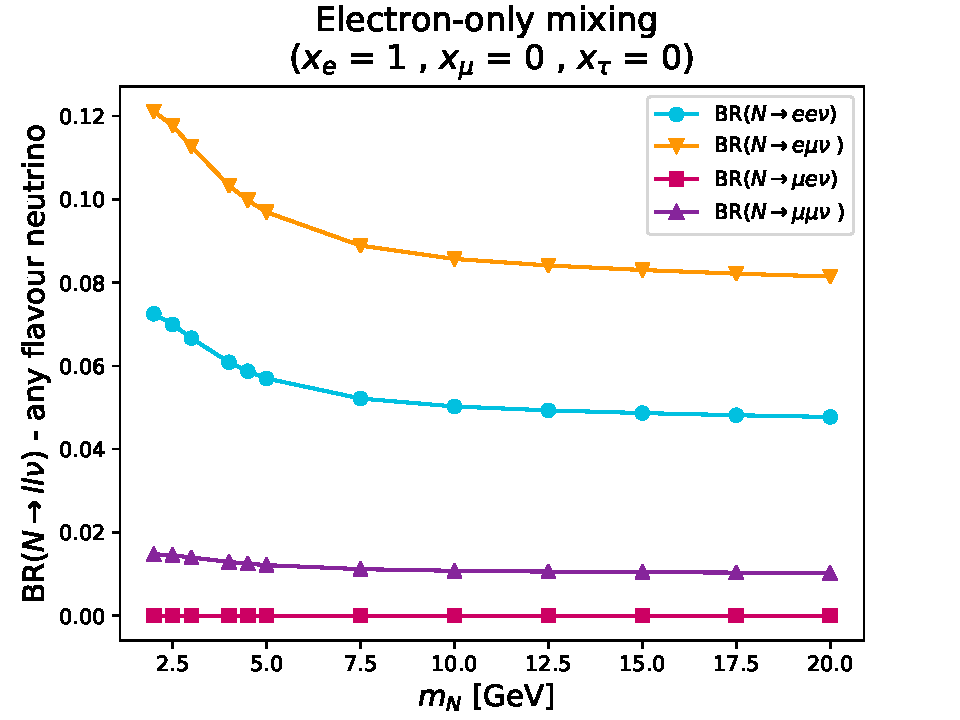
\includegraphics[width=.5\textwidth]{figures/theory/br_e_only.pdf}}
    \subfloat[1SFH($\mu$)]{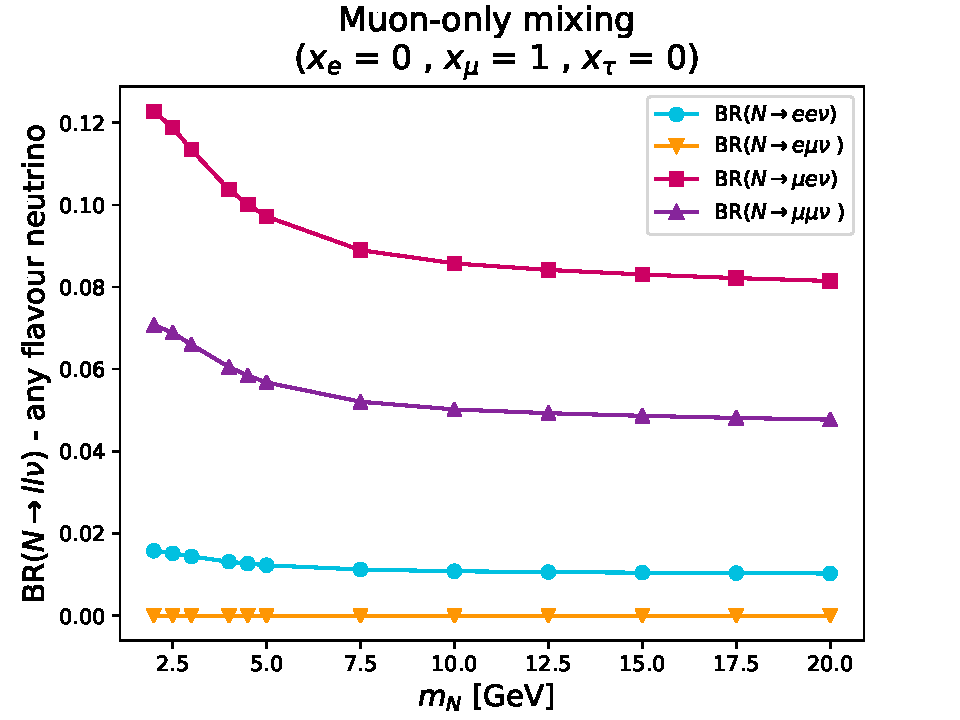
\includegraphics[width=.5\textwidth]{figures/theory/br_mu_only.pdf}}\\
    \subfloat[2QDH(IH)]{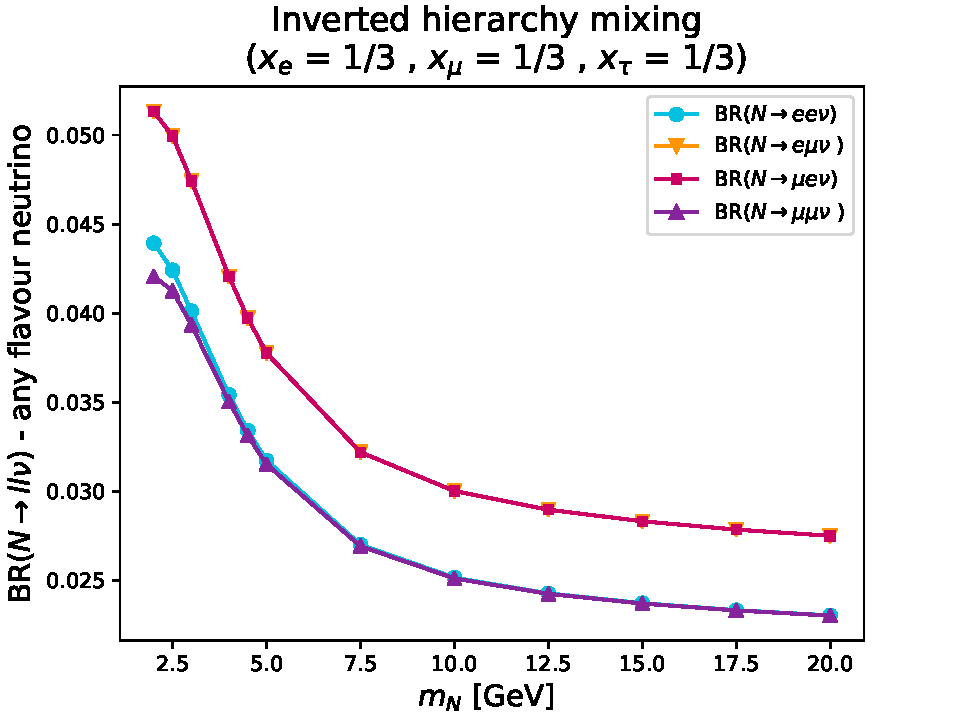
\includegraphics[width=.5\textwidth]{figures/theory/br_IH.pdf}}
    \subfloat[2QDH(NH)]{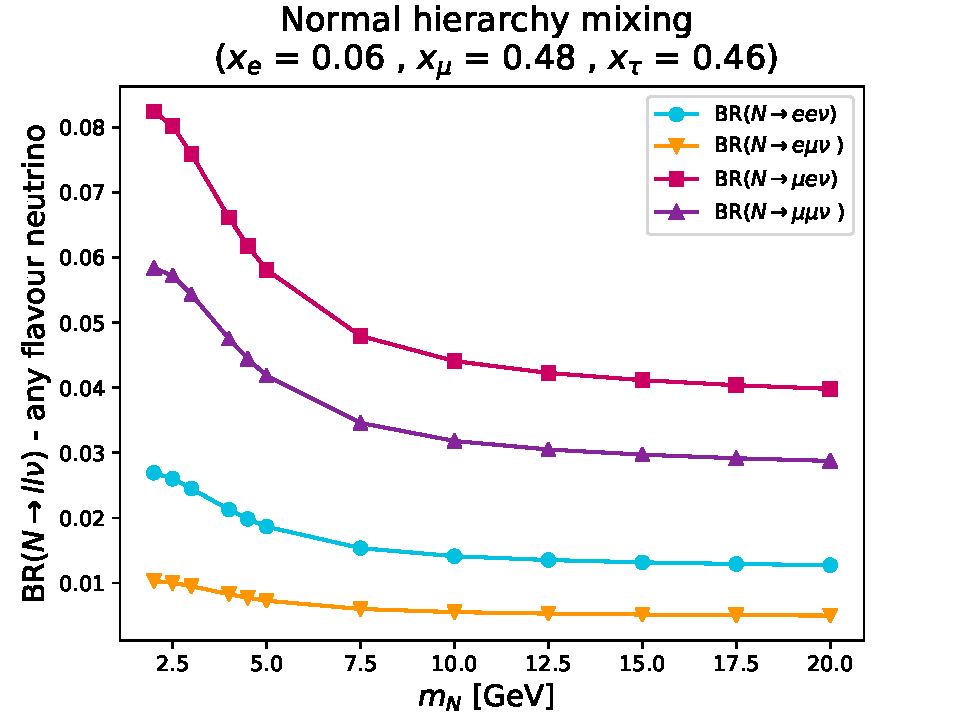
\includegraphics[width=.5\textwidth]{figures/theory/br_NH.pdf}}
    \caption{$BR(N\to \ell\ell\nu)$ for the four benchmark models. For each scenario, the branching ratio is shown for $N\to ee\nu$ (blue), $N\to e\mu\nu$ (orange),  $N\to \mu e\nu$ (pink), and $N\to\mu\mu\nu$ (purple) decays. The $y$-axis range is adjusted for each model for clarity.~\cite{Trischuk:2806047}}
    \label{fig:branching_ratio}
\end{figure}

The differences in $BR(N\to\ell_\beta\ell_\gamma\nu)$ and $BR(N\to\ell_\gamma\ell_\gamma\nu)$ are due to interference effects between the charged and neutral current mediated decays. For muon-only mixing HNL, $N\to e\mu\nu$ is forbidden and $N\to ee\nu$ is only possible from neutral current decays. Similarly, for electron-only mixing, $N\to \mu e\nu$ is forbidden and $N\to \mu\mu\nu$ is possible only from neutral current decays. Since the NH mixing favors a coupling to the muon neutrino, its branching ratios are similar to that of the muon-only mixing scenario, except that all final states have non-zero contributions. The IH mixing favors all final states equally, with the difference coming from the interference between the charged and neutral currents.

The proper lifetime of the HNL, $\tau_\mathrm{HNL}$, depends on the mass of the HNL, \mhnl, and the strength of the coupling to SM neutrinos, $U$,~\cite{PhysRevD.29.2539}:
\begin{equation}
    \tau_\mathrm{HNL} \propto \frac{1}{\mhnl^5 |U|^2}.
\end{equation}

The constant of proportionality depends on the benchmark model being considered. For very small couplings, the lifetime is large enough that it can be resolved by the detectors of the ATLAS experiment. The coupling $|U|^2$ can be analytically computed for a given generated mass and lifetime in a simplified Fermi theory computation~\cite{Bondarenko2018}, approximating the HNL production and decay as a four-fermion interaction vertex. After considering all decay widths and summing over the possible decay channels, the obtained mixing angle, $|U|^2$ as a function of the HNL mass for the muon-only mixing scenario is shown in~\cref{fig:mixing_angle} to yield three representative HNL lifetimes. As stated, the shape of the functional relation between $|U|^2$ and \mhnl is identical for the models considered, and the proportionality constant has similar magnitudes for them.

\begin{figure}[!ht]
    \centering
    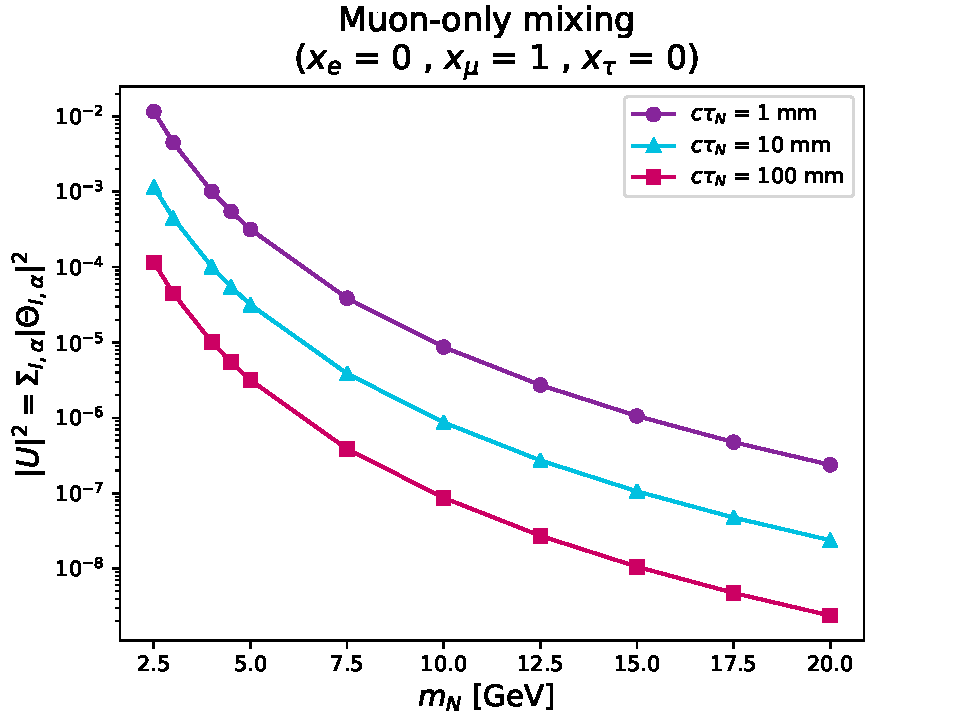
\includegraphics[width=.6\textwidth]{figures/theory/theta_Uu.pdf}
    \caption{The total mixing angle $|U|^2$ as a function of the HNL mass (\mhnl or $m_N$) for the 1SFH($\mu$) model shown for the \ctau values 1 mm (purple), 10 mm (blue), and 100 mm (pink)).~\cite{Trischuk:2806047}}
    \label{fig:mixing_angle}
\end{figure}
